\nnarticleheader{Polar Art}{Joey Kauffman, Haverford '23}

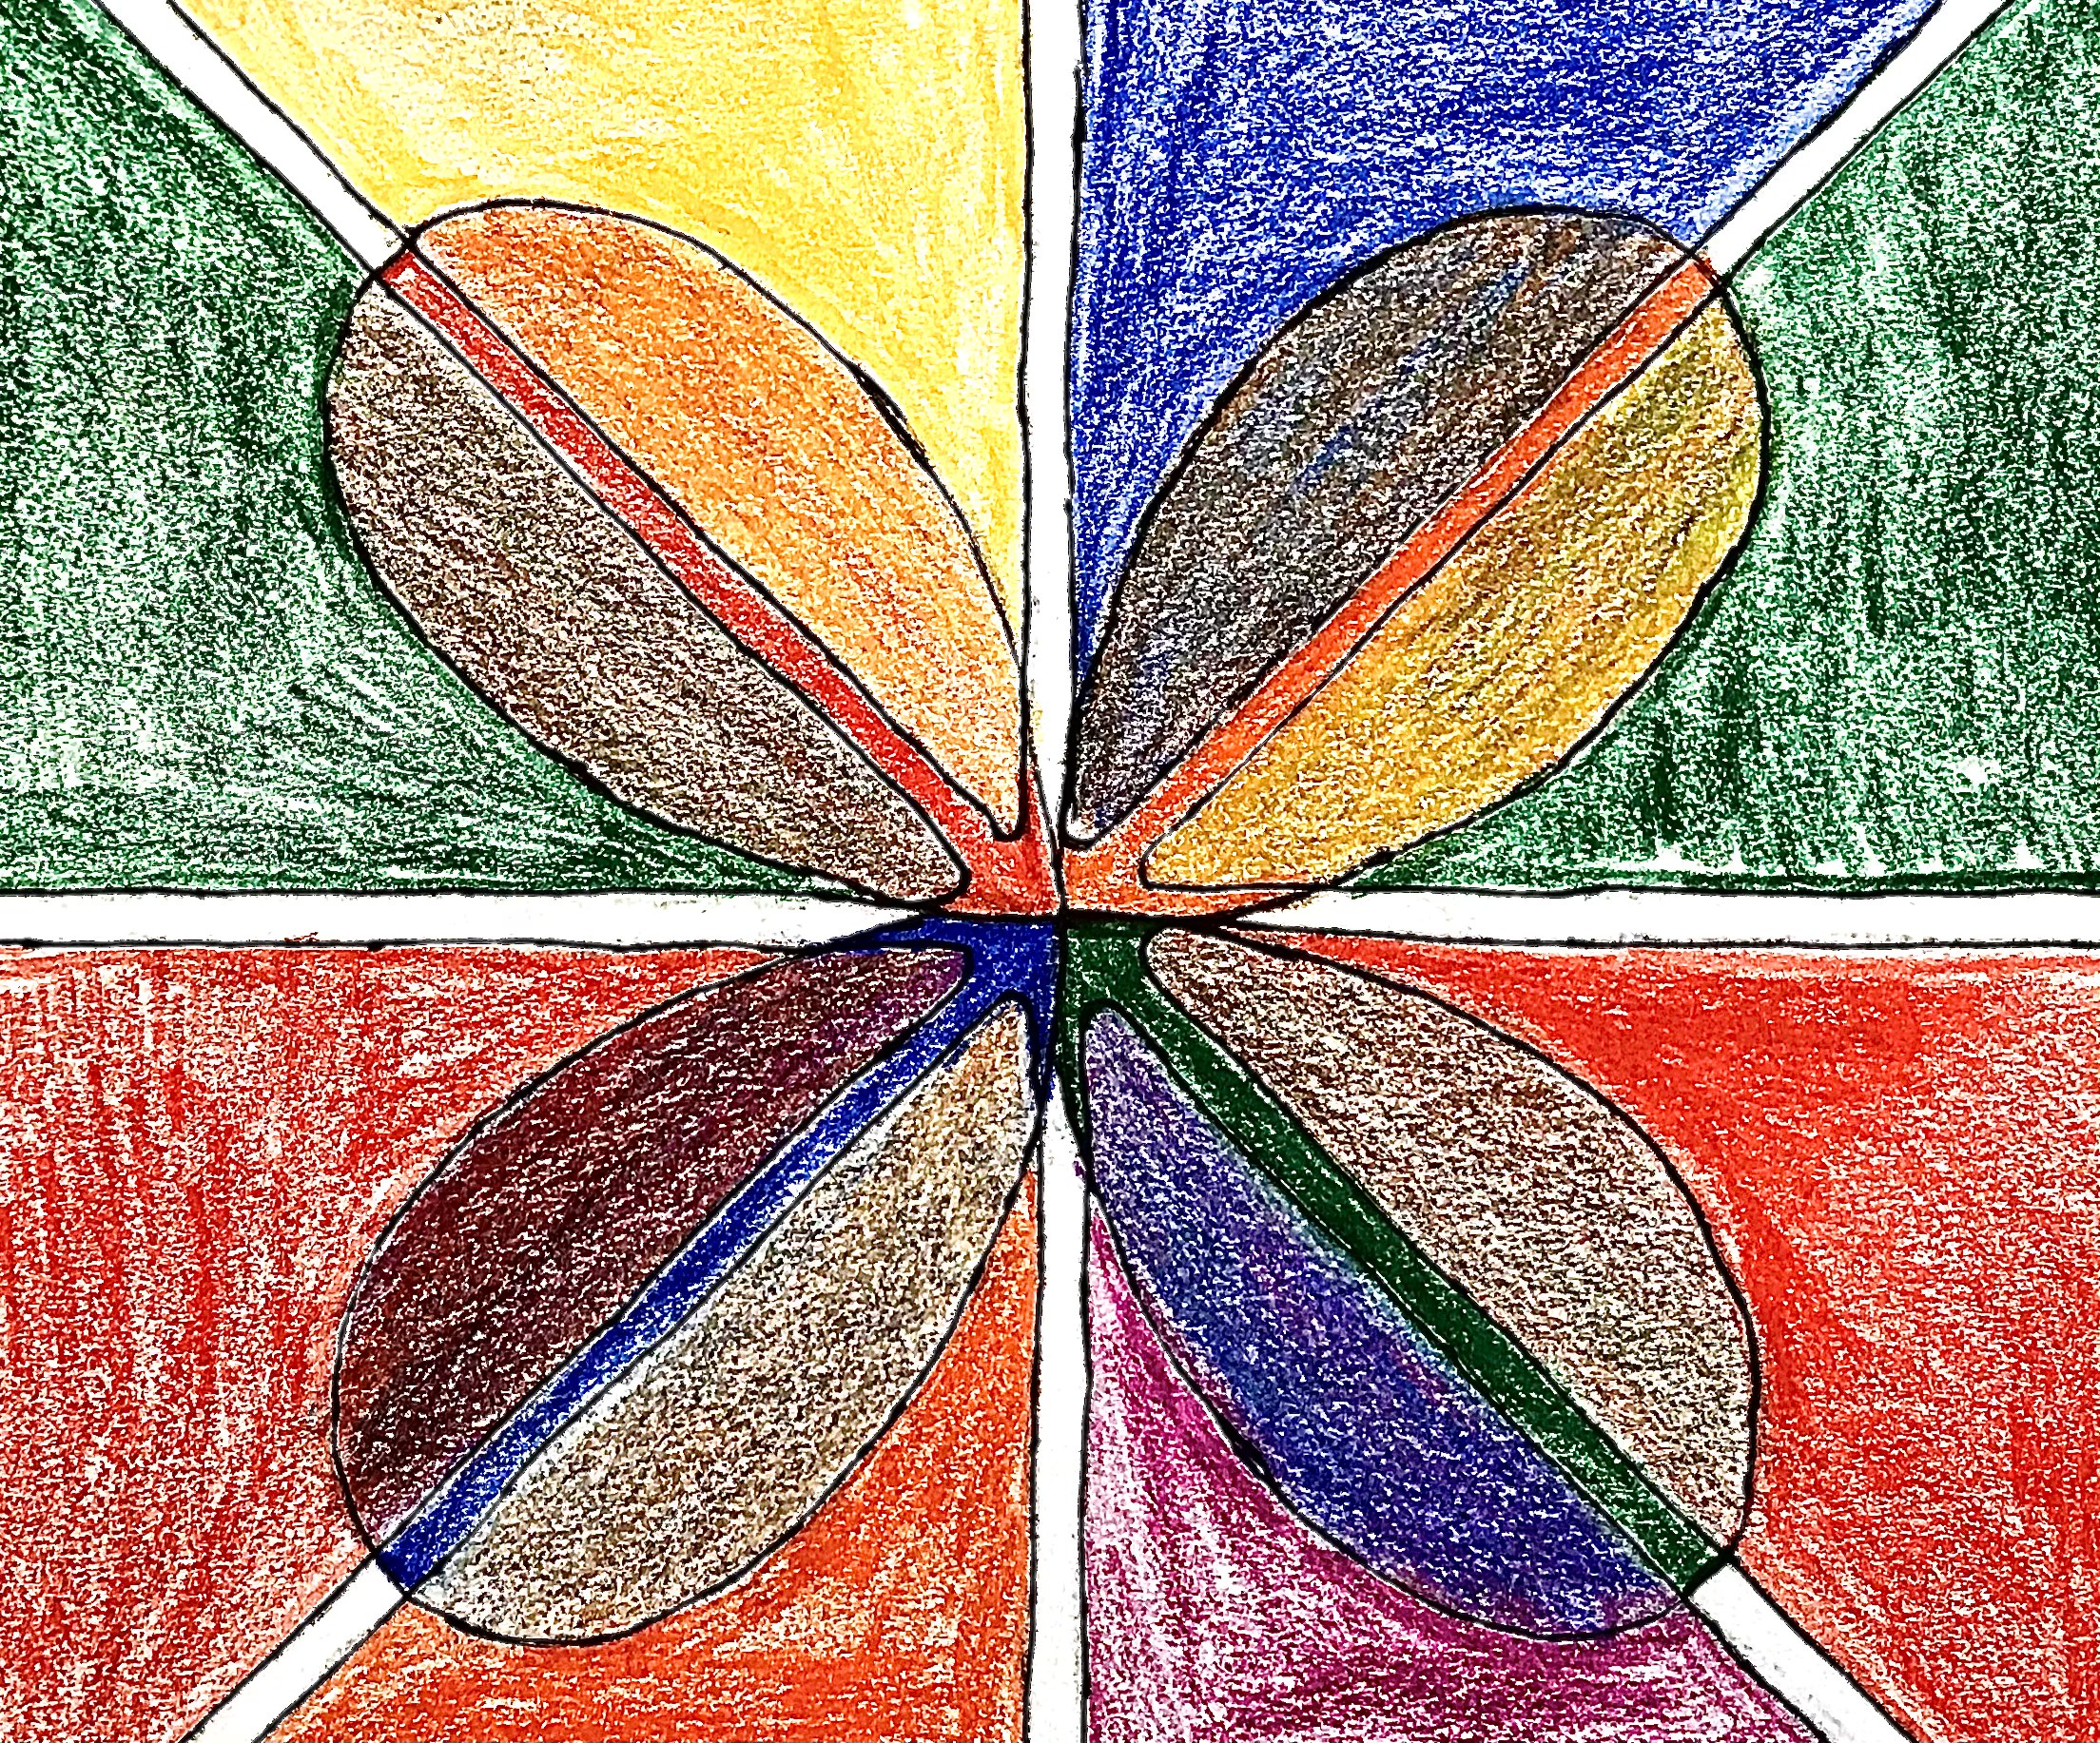
\includegraphics[width=0.9\textwidth]{kauffman_final_art.jpg}

\noindent
\textbf{Introduction}

When I began to play around with polar equations at the beginning of this project, the polar curve
\begin{align*}
    r = \frac{1}{\sin(4\theta)}
\end{align*}
was the first curve that really caught my eye. Artistically, the curve is appealing because of its eight distinct ``parts'' that all radiate from the origin/pole.\footnote{Later in the write-up, I refer to these ``parts'' as ``shards''.} When looking at the graph for this curve, it’s almost as if one can either focus on the eight ``parts'' of the curve---which look like shards that angle towards the origin, hit a radius length of 1, and fly back to the outer depths of the graph---or, one can see the distance between the shards, which look like rays of mathematical validity---eight sunbeams, each one devoted to never dividing by zero.

However, the curve is just as interesting mathematically as it is artistically. Firstly, the graph has asymptotes at any $\theta$ value that would cause $\sin(4\theta)$ to equal zero, because if $\sin(4\theta)$ were equal to zero, then the equation would produce an undefined value. These values of $\theta$ that the curve excludes are $0$, $\nicefrac{\pi}{4}$, $\nicefrac{\pi}{2}$, $\nicefrac{3\pi}{4}$, $\pi$, $\nicefrac{5\pi}{4}$, $\nicefrac{3\pi}{2}$, and $\nicefrac{7\pi}{4}$. You may notice that these are eight values in total. This is the reason why there are eight ``shards'' to the curve. Another interesting part about this curve is that the equation never has an $r$ value smaller than 1. This is because for that to happen, the output of $\sin(4\theta)$---the denominator of the equation---would need to be greater than one. This is impossible because $\sin(4\theta)$ depicts the unit circle with a radius of one.

To complement this graph, I wanted to find a curve that intersected large parts of the ``shards'' of the $r = \nicefrac{1}{\sin(4\theta)}$ graph. The curve
\begin{align*}
    r = 10\sin(2\theta)
\end{align*}
did this. This curve intersects all eight of the parts of the $r = \nicefrac{1}{\sin(4\theta)}$ graph, resulting in 16 intersections. To make it even more interesting, only 8 of these intersections are real solutions. The reason for this is that during the intervals of $\theta = (\frac{\pi}{4}, \frac{\pi}{2}), (\frac{3\pi}{4}, \pi), (\frac{5\pi}{4}, \frac{3\pi}{2}), and (\frac{7\pi}{4}, 2\pi)$, the value of $r$ for $r = \nicefrac{1}{\sin{4\theta}}$ is negative, which flips the points 180 degrees about the origin. An example is an \begin{wrapfigure}{l}{0.55\textwidth}
    \centering
    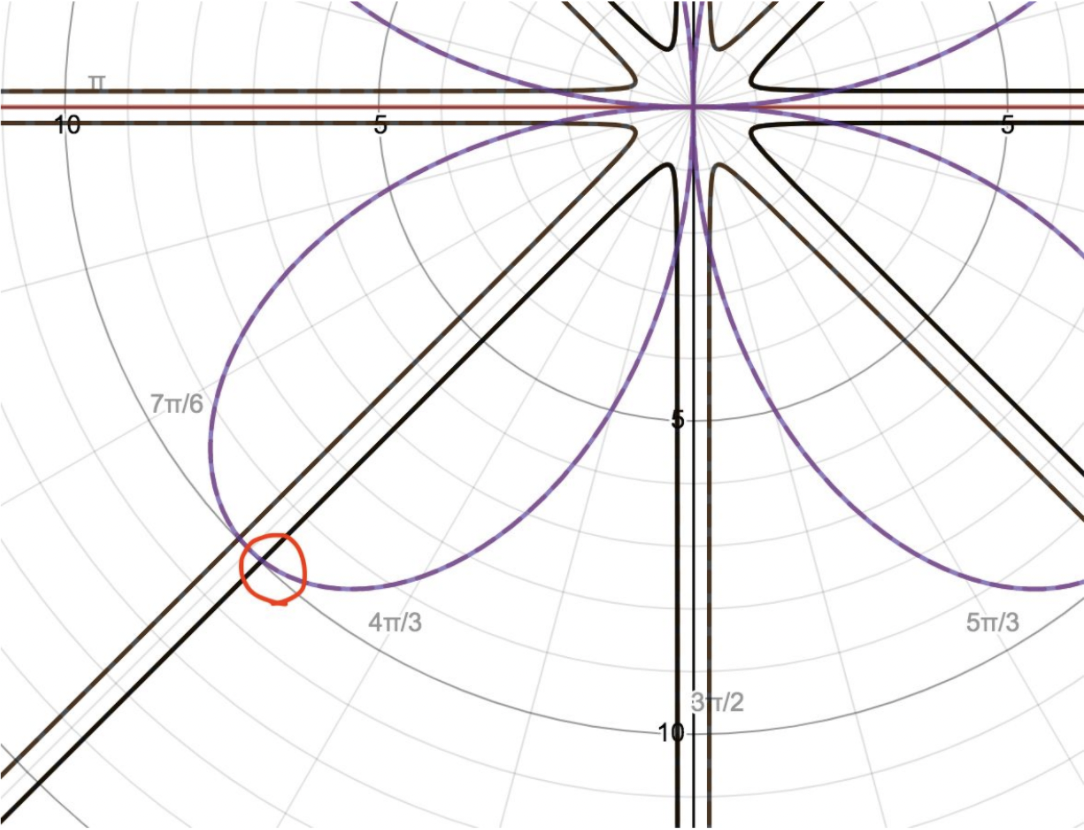
\includegraphics[width=0.55\textwidth]{kauffman_desmos_1.png}
\end{wrapfigure} intersection point in the third quadrant, as seen on the left. $r = \nicefrac{1}{\sin{4\theta}}$ intersects this point shortly after $\theta = \nicefrac{\pi}{4}$ because this leads to a negative $r$ for $r = \nicefrac{1}{\sin{4\theta}}$. However, $r = 10\sin(2\theta)$ intersects this point shortly after $\theta = \nicefrac{5\pi}{4}$, meaning that they do not intersect the point at the same time---not a solution.

This means that, going counter-clockwise around the polar graph, there will be two solutions, then two non-solution intersections, then two solutions, etc. I was able to verify this by looking at the graphs of $y = \nicefrac{1}{\sin{4\theta}}$ and $y = 10\sin(2\theta)$ \begin{wrapfigure}{l}{0.15\textwidth}
    \centering
    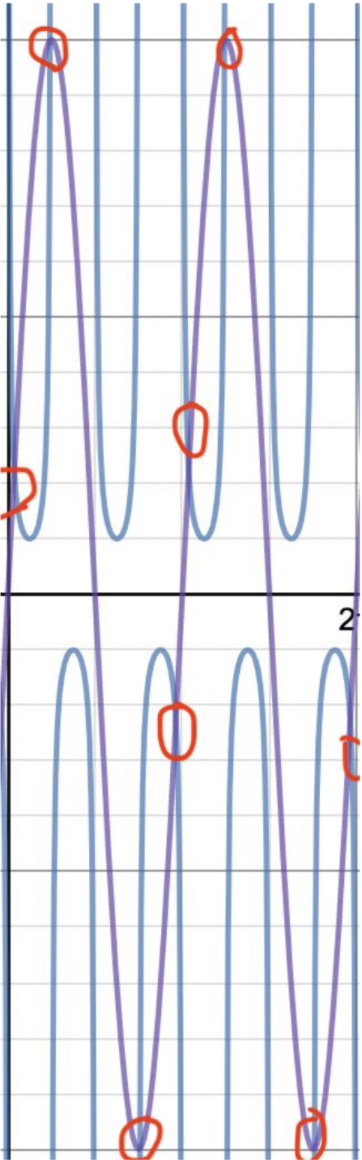
\includegraphics[width=0.15\textwidth]{kauffman_desmos_2.png}
\end{wrapfigure} in Desmos, as seen on the left. We know this graph will only give real solutions at points of intersections because we are graphing the functions in the Cartesian plane, replacing $r$ with $y$. In the Cartesian plane, there is no ambiguity---an intersection is always a solution. From this graph, we can see that there are 8 solutions in the period of $0$ to $2\pi$ (after that, the solutions begin repeating). The eight solutions are $(0.114, 2.266)$, $(0.76, 9.987)$, $(2.318, -9.987)$, $(3.027, -2.266)$, $(3.256, 2.266)$, $(3.902, 9.987)$, $(5.523, -9.987)$, and $(6.169, -2.2657)$.
\\\\
\noindent
\textbf{Attempting to Find an Analytical Solution}

Before I cover how I represented these solutions with color, I would like to present my attempt to solve this analytically, not using Desmos. First, I set
\begin{align*}
    \frac{1}{\sin{4\theta}} = 10\sin{2\theta}.
\end{align*}
Then, I defined a variable $t = 2\theta$. The equation now looked like \begin{align*}
    \frac{1}{\sin{2t}} = 10\sin{t}.
\end{align*}
Then, because $\sin{2a} = 2\sin{a}\cos{a}$, I made the equation
\begin{align*}
    \frac{1}{2\sin{t}\cos{t}} = 10\sin{t}.
\end{align*}
Next, I cross-multiplied to get
\begin{align*}
    20\sin^2{t}\cos{t} = 1,   
\end{align*}
and then
\begin{align*}
    \sin^2{t}\cos{t} = \frac{1}{20}.   
\end{align*}
Then, because $\sin^2{a} = 1 - \cos^2{a}$, we can write
\begin{align*}
    \left(1 - \cos^2{t}\right)\cos{t} = \frac{1}{20}   
\end{align*}
and
\begin{align*}
    \cos{t} - \cos^3{t} = \frac{1}{20}.   
\end{align*}
This is when I hit a roadblock and couldn't think of anything to do since the cosines have different exponents.

\noindent
\textbf{Coloring the Graph}

Now, when it came time to depict the intersections with color, I wanted to represent the non-solution intersections by using the blackish-brown result of mixing two complementary colors and the solutions by using a more pleasant mix of two primary or secondary colors.

There are four ``leaves'' of the $r = 10\sin{2\theta}$ equation, and I made two opposing leaves red and green (complements) and the other two opposing leaves orange and blue (complements). Now, if the ``shard'' of the $r = \nicefrac{1}{\sin(4\theta)}$ intersected with one of the four leaves and was not a solution, I colored the ``shard'' the complement of the leaf, which is the color of the opposing leaf. When the ``leaf'' and the ``shard'' overlapped, a brownish color formed, signifying that their intersection was not a solution to the equation.

However, if the intersections between the two equations were solutions, I wanted the color formed to be a pleasant primary or secondary color. I applied a system of choosing the color of the ``shard'' in this scenario so that the color progression would have some sort of order. The system was that, in a color wheel of only primaries and secondaries, I took the color of the leaf---the $r = 10\sin{2\theta}$ equation---and I went two spaces clockwise in the color wheel and made that the color of the shard---the $r = \nicefrac{1}{\sin(4\theta)}$ equation. When I did this, the color in between the color of the ``shard'' and the color of the ``leaf'' in the color wheel would form when the ``shard'' and ``leaf'' overlapped. For example, when there was a red leaf, I made the ``shard'' yellow, and that made the space where they intersected orange. When there was a blue leaf, I made the ``shard'' red, and that made the intersection space violet.

This ended up giving some sort of pattern to the space where there were solutions, yet I must acknowledge the shortcomings of this method. It is not very clear where the intersections are from the way I did it. All you can really see is that the two functions sometimes form a brown color in the space where they intersect, and they sometimes form a different, more pleasant color; the actual points of intersection are not highlighted at all. From my perspective, this is its greatest limitation; however, I do believe that my polar art effectively contrasts the areas of intersection that are solutions with the areas of intersection that are not solutions.
